\chapter{Blackboard}

\section{Summary}
Das Blackboard Pattern ist nützlich bei Problemen für die keine deterministischen Lösungsstrategien bekannt sind. Dabei kombinieren mehrere spezialisierte Teilsysteme ihr Wissen um eine annähernde Lösung zu kreieren. 
\section{Context}
Eine unreife Domäne in der keine eindeutige Herangehensweise zu einer Lösung bekannt oder möglich ist.

\section{Problem}
Das Blackboard Pattern kümmert sich um Probleme bei denen es keine praktikable deterministische Lösung für die Transformation von Rohen Daten nach High-Level Datenstrukturen (Tabellen, Diagramme, etc.) gibt. Solche Probleme charakterisieren sich dadurch, dass wenn man Sie in Teilprobleme unterteilt, diese sich über mehrere Kompetenzbereiche verteilen. Es gibt dabei keine vordefinierte Strategie, wie die Teilprobleme ihr Wissen kombinieren sollten.\\
Folgende Forces beeinflussen die Lösungen zu solchen Problemen:
\begin{itemize}
	\item Ein komplettes durchsuchen der Lösung ist nicht innert brauchbarer Zeit möglich
	\item Experimentieren mit verschiedenen Algorithmen für denselben Subtask notwendig
	\item Verschiedene Algorithmen lösen das selbe Problem
	\item Input, Zwischenresultate und Endresultate haben verschiedene Formate
	\item Ein Algorithmus arbeitet auf den Resultaten eines anderen Algorithmus
	\item Ungenaue Lösung und Näherungswerte sind oft einbezogen
	\item Zerlegte Algorithmen bringen eventuell Parallelität ein 
\end{itemize}

\section{Solution}
Die Idee hinter der Blackboard Architektur ist eine Sammlung von unabhängigen Programmen die zusammen auf einer gemeinsamen Datenstruktur arbeiten. Jedes Programm ist darauf spezialisiert ein gewisses Teilproblem zu lösen, es arbeitet komplett unabhängig von den andern. Es gibt auch keine vordefinierte Reihenfolge in der sie ablaufen, die Reihenfolge wird vom aktuellen Prozessstatus bestimmt. Eine zentrale Kontrollkomponente, "Moderator" genannt, evaluiert den aktuellen Prozessstatus und Koordiniert die Programme. Dieses Daten gesteuerte System nennt man "opportunistic problem solving".\\
Während dem Problemlösungsprozess arbeitet das System mit Teillösungen welche kombiniert, geändert und verworfen werden. Das Set aller möglichen Lösungen wird "solution space" genannt und ist nach Abstraktionsleveln organisiert.\\
Der Name Blackboard kommt von der Ähnlichkeit zur Situation in der mehrere Menschen um ein richtiges Blackboard stehen und versuchen zusammen ein Problem zu lösen.

\subsection{Structure}
Für das Blackboard Pattern werden drei verschiedene Komponenten benötigt, das Blackboard selbst, eine Sammlung von "Knowledge Sources" und eine "Control" Komponente. Im folgenden werden diese kurz beschrieben.
\paragraph{Blackboard}
Das Blackboard dient als zentraler gemeinsamer Datenspeicher. Der Begriff "Vocabulary" wird für die Sammlung von Datenelementen verwendet die auf dem Blackboard erscheinen können. Vom Blackboard wird ein Interface angeboten das allen "Knowledge Sourcen" ermöglicht darauf zu schreiben und zu lesen. Lösungen die während dem Problemlösungsprozess entstehen werden auf das Blackboard gelegt, sie nennt sie "Hypothesis". Eine solche Hypothese hat ein Abstraktionslevel welcher die konzeptionelle Distanz vom Input darstellt. Ein tiefer Abstraktionslevel bedeutet man hat eine Repräsentation die näher beim Input ist, ein hoher dass man näher beim Output ist.
\paragraph{Knowledge Sources}
Knowledge Sources sind Subsysteme die spezifische Aspekte des Gesamtproblems lösen. Keine Knowledge Source kann das Gesamtproblem selbst lösen, dies ist nur durch zusammenführen aller Teillösungen möglich. Sie kommunizieren nicht direkt untereinander, sondern schreiben und lesen nur auf dem Blackboard. Jede Knowledge Source muss die Bedingungen kennen unter welchen sie zur Lösung beitragen kann, deshalb werden sie unterteilt in einen Condition und einen Action Teil. Der Condition Teil evaluiert anhand dem das auf dem Blackboard steht, ob zur Lösung beigetragen werden kann. Der Action Teil produziert dann eine neue Teillösung.
\paragraph{Control}
Die Control Komponente läuft in einer Schlaufe die den Inhalt des Blackboards überwacht und entscheidet was als nächstes ausgeführt werden soll. Die Entscheidungen basieren eventuell auf Berechnungen die von speziellen Knowledge Sources ausgeführt werden.

Die folgende Grafik zeigt das Zusammenspiel der einzelnen Komponenten.
\begin{figure}[H]
	\centering
	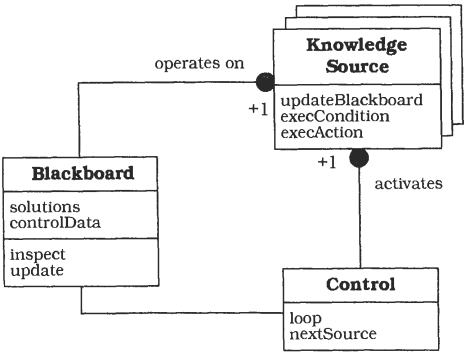
\includegraphics[width=0.6\textwidth]{figures/02-blackboard-1}
	\caption{Zusammenspiel der Blackboard Komponenten}
\end{figure}

\section{Consequences}
\begin{itemize}
    \pro{Experimentieren mit verschiedenen Algorithmen}
    \pro{Verschiedene Kontrollheuristiken können verknüpft werden}
    \pro{Unterstützt Wartbarkeit und Veränderbarkeit}
    \pro{Wiederverwendbare Wissensquellen}
    \pro{Fault Tolerance und Robustness}
    \con{Schwierig zu testen}
    \con{Keine gute Lösung garantiert}
    \con{Schwierig eine gute Kontrollstrategie zu entwickeln}
    \con{Tiefe Effizienz}
    \con{Hoher Entwicklungsaufwand}
    \con{Kein Support für Parallelität}
\end{itemize}

\section{Known Uses}
\begin{itemize}
	\item CRYSALIS (X-Ray Bilderkennung)
	\item HEARSAY-II (Spracherkennung)
	\item HASP/SIAP (Erkennung von gegnerischen U-Booten)
	\item TRICERO (Monitoring von Flugzeug Aktivitäten) 
\end{itemize}

\section{Relationships}
\begin{itemize}
	\item \textit{Keine} 
\end{itemize}

\section{Exam Questions}
\begin{itemize}
  \item Behauptung: dies ist eine Behauptung? (Lösung)
    \item Frage: Dies ist eine Frage? (Lösung)
\end{itemize}
